

% Other Frameworks Chapter: Expanded and Enhanced
\subsection*{1. Introduction to Alternative Threat Modeling Frameworks}
Threat modeling is a diverse and continually evolving discipline, with multiple frameworks developed to address the unique needs of different organizations, industries, and regulatory environments. While STRIDE and PASTA are among the most widely adopted methodologies, several other frameworks offer valuable perspectives and tools for managing risk. This chapter explores four important alternatives—Trike, VAST, OCTAVE, and OWASP—providing technical definitions, strengths, limitations, and practical guidance for their application\cite{owasp,nist800154}.

\subsection*{2. Trike}
Trike is a risk management and threat modeling framework that emphasizes the definition of acceptable risk and the generation of threat models based on system requirements\cite{uceda2015}. It employs three core models:
\begin{itemize}
	\item \textbf{Requirement Model:} Defines what is allowed and expected in the system.
	\item \textbf{Attack Model:} Identifies potential failures and maps attacker actions to system components.
	\item \textbf{Risk Model:} Quantifies the impact and likelihood of threats to support risk-based decision making.
\end{itemize}
Trike’s strengths lie in its quantitative approach and strong focus on requirements, making it particularly useful for auditors and risk managers. However, its complexity and limited tool support can make it less intuitive for developers and teams new to threat modeling.

\subsection*{3. VAST (Visual, Agile, and Simple Threat)}
VAST is designed for scalability and integration with agile and DevOps workflows. It uses visual diagrams to model both application and operational threats, making it suitable for large organizations with complex systems. VAST emphasizes automation and continuous threat modeling, allowing teams to adapt quickly to changes in the environment and development process\cite{owasp}. Its strengths include scalability, visual clarity, and seamless integration with CI/CD pipelines. The main limitation is that it provides less detailed adversary simulation compared to frameworks like PASTA.

\subsection*{4. OCTAVE (Operationally Critical Threat, Asset, and Vulnerability Evaluation)}
Developed by Carnegie Mellon, OCTAVE focuses on organizational risk and asset-based analysis. It aligns security with business objectives and is often applied at the enterprise level, where strategic considerations are paramount\cite{nist800154}. OCTAVE’s strengths include its business alignment, asset-centric approach, and strategic focus. However, it offers less technical detail and is not ideally suited for application-level threat modeling.

\subsection*{5. OWASP Threat Modeling}
OWASP provides a wealth of resources, including the Threat Modeling Cheat Sheet, which offers practical guidance, checklists, and templates. OWASP’s approach is community-driven and emphasizes actionable steps for developers and security teams\cite{owasp}. Its strengths are practicality, widespread adoption, and the availability of open-source resources. The main limitation is that OWASP does not offer a formal framework, but rather a collection of best practices and tools.

\subsection*{6. Framework Comparison Table}
The following table compares the major threat modeling frameworks, highlighting their focus, best use cases, and limitations:
\begin{table}[H]
\centering
\begin{tabular}{|l|l|l|l|}
\hline
		extbf{Framework} & \textbf{Focus} & \textbf{Best For} & \textbf{Limitation} \\
\hline
STRIDE & Application threats & Development/design teams & Less business focus \\
PASTA & Risk/attacker simulation & Regulated, high-value environments & Resource intensive \\
Trike & Risk quantification & Auditors, risk managers & Steep learning curve \\
VAST & Scalability & Large, agile organizations & Less adversary detail \\
OCTAVE & Organizational risk & Enterprise, strategy & Not application-level \\
OWASP & Practical steps & Developers, SMEs & Not a full framework \\
\hline
\end{tabular}
\caption{Comparison of Threat Modeling Frameworks\cite{owasp,uceda2015,nist800154}}
\end{table}

\subsection*{7. Visual Comparison and Practical Guidance}
\begin{figure}[H]
	\centering
	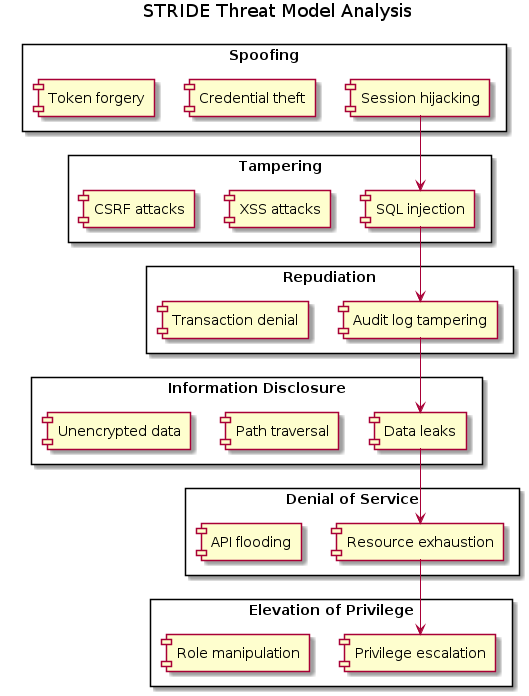
\includegraphics[width=0.8\textwidth]{images/stride-analysis}
	\caption{Visual Comparison of Threat Modeling Frameworks}
\end{figure}

\subsection*{8. Academic Perspective and Further Reading}
For deeper understanding, refer to:
\begin{itemize}
	\item Tony UcedaVélez and Marco M. Morana, "Risk Centric Threat Modeling" (Wiley, 2015)
	\item Adam Shostack, "Threat Modeling: Designing for Security" (Wiley, 2014)
	\item NIST SP 800-154: Guide to Data-Centric System Threat Modeling
	\item OWASP Threat Modeling Cheat Sheet
\end{itemize}
